\section{Appendix: Neutrino Interactions and Uncertainties}\label{sec:nu-osc-11} \label{sec:physics-lbnosc-nuint-app}
%{\it Assigned to:} {\bf Kevin McFarland}

%{\it Assigned to:} {\bf Kevin McFarland} with contributions from Kendall and the DuneReweight group. This section has a description of event generator used, justify choices of model and a description of Dune Reweight and treatment of the uncertainties.  This will be organized by reaction type or effect, preferably with overarching categories as subsections.

\subsection{Interaction Model Summary}

The model proposed herein generally factorizes the neutrino
interaction on nuclei into an incoherent sum of ``hard scattering'' neutrino interactions with the single nucleons in the nucleus. The effect of the nucleus is implemented as
initial and final state interaction effects, with some (albeit few) nucleus-dependent hard scattering calculations. Schematically, we express this concept as $\text{Scattering Process} = \text{Initial State} \otimes \text{Nucleon Interaction} \otimes \text{Final State Propagation}$.


By ``initial state'' effects, we usually mean a description of the momentum and position distributions of the nucleons in the nucleus, kinematic modifications to the final state (such as removal energy, sometimes described as a ``binding energy''), and Coulomb effects.   The concept of ``binding energy'' indicates that the struck nucleon may be off the mass-shell inside the nucleus.
\Dword{fsi} %``Final state interactions'' (FSI) 
refer to the propagation and interaction of hadrons produced in the nucleon interaction through the nucleus. The \dword{fsi} alter both the momentum and energy of the recoiling particles produced in the final state, and may also alter their identity and multiplicity in the case of inelastic reinteractions (e.g., in a nucleus a hadron may be absorbed, rescattered, or create a secondary hadron).  The \dword{fsi} model implemented in the \dword{genie}, \dword{nuwro}, and \dword{neut} neutrino interaction generators is a semi-classical cascade model (or in the case of \dword{genie}'s $hA$ model a single step scaled model), based on hadron-nucleus and hadron-nucleon scattering data and theoretical corrections.  \dword{gibuu}, another available generator, uses a full particle transport model, including support for off-shell hadrons in the nuclear medium.

Generators vary in their attempts to accurately model the largely undetected final state ``spectator'' nuclear system.  The nuclear system can carry away significant undetected momentum---hundreds of MeV is not unusual---in the form of one or more heavy, non-relativistic particles.  These particles typically carry off very little kinetic energy; however they can absorb of order tens of MeV of energy from the initial state from breakup or excitation of the target nucleus.  Most of this energy and momentum will typically be invisible to the detector.
%KSM says, I'm not sure who added this, but the few 100 MeV momentum is the size of the Fermi momentum, the "little kinetic energy" is p^2/2M_nucleus~(20/A) MeV, and the
%KSM\fixme{Add citations for spectator nucleus if possible}

The factorization outlined above is not present in all parts of the model.  Most modern generators include ``2p2h'' (two particle, two hole) interactions that model meson exchange processes and scattering on highly correlated pairs of nucleons in the nucleus.  These interactions are often implemented as another process that incorporates both hard scattering and initial state effects in processes that create multiple final state nucleons, with a different prescription for different nuclei.
Neutrino scattering on atomic electrons and the coherent production of pions (which scatters off the entire nucleus) also
do not follow this factorization.

The interaction model and its variations are implemented in the  \dword{genie} generator.  The fixed version of \dword{genie} used for this report, v2.12.10\footnote{At the time of the development of this report, \dword{genie} 3 had just recently been released (October 15, 2018).  However, at the time of that release, there was no documentation of the tunes, and the code required to implement uncertainties had also not been released; therefore, it was not feasible to use \dword{genie} 3 for this work.}, will not contain all of the possible cross section variations which need to be modeled.  Therefore, the variations in the cross sections to be considered are implemented as some combination of: \dword{genie} weighting parameters (sometimes referred to as ``\dword{genie} knobs''), {\it ad hoc} weights of events which are designed to parameterize uncertainties or cross section corrections currently not implemented within \dword{genie}, and as discrete alternative model comparisons, achieved through alternate generators, alternate \dword{genie} configurations, or custom weightings.

Discrete alternative model comparisons are valuable, but are used sparingly in this work due to finite computational resources and ease of interpretation. The approach taken was to identify classes of uncertainties and provide generous uncertainties intended to span a reasonable range of alternate models. Using the alternate model as mock data either provides a closure test, or a mechanism by which to inflate uncertainties. Most of the alternate models in other generators (GiBUU, NEUT and NuWro) or alternate configurations of \dword{genie} are expected to be covered by the uncertainties described here.

%It is not guaranteed that the alternate models will be covered by the chosen systematic uncertainty, but analysis  of alternate models can be computationally slow and interpretation not easy; there may be artificial reasons (e.g. a given generator's implementation choice ) which can create unexpected effects.

For this work, we chose one particular discrete alternate model as a source of uncertainty, inspired by differences in models but which has a well defined implementation and interpretation; it is described in Section~\ref{sec:fsi}. The most problematic feature of an interaction model for any oscillation analysis is if the model uncertainties are incomplete in the association between reconstructed observables and true neutrino energy. A special mock data sample was created which preserved the same observables for on-axis samples as the default sample, but which significantly modifies the observable--true energy relationship.
%This isolates one of the fundamental issues, which is that all tests of the relationship to true neutrino energy via observables have so far been largely indirect and averaged over a broad

%\fixme{ KM outline:}
%- Future work on DUNE will develop better machinery for alternate generators; this is a computational and technical challenge faced by many experiments;
%-- LBNC may not accept "computing limitations" so trying to finesse this
%- Alternate generators provide a closure test of the weighting scheme and/or a new uncertainty
%-- NEUT/NuWro variations expected to be covered by current parameterization, but generally,
%-- the uncertainties generally span the availible GENIE alternate configurations. (non-reweightable knobs that are  implemented, e.g., formation zone and other hadronization uncertainties-- not quite)
%--But, there can be artificial reasons why a particular generator-generator comparison may not reflect error (e.g. bug in implmentatin). We can't generally know how to interpret the results, so they are not considered here.

%- One single important case-- and this is the most worrysome case which the alternate generators embody:  This mock data sets modify the reconstructed to true neutrino energy relationship, while preserving the outgoing final state particle kinematics. This isolates one of the fundamental issues, which is that all tests of the relationship to true neutrino energy via observables have so far been largely indirect and averaged over a broad flux.
\subsection{Interaction Model Uncertainties}

The interaction uncertainties are divided into seven roughly exclusive groups: (1) initial state uncertainties, (2) hard scattering uncertainties and nuclear modifications to the quasielastic process, (3) uncertainties in multinucleon (2p2h) hard scattering processes, (4) hard scattering uncertainties in pion production processes, (5) uncertainties governing other, higher $W$ and neutral current processes, (6) final state interaction uncertainties, (7) neutrino flavor dependent uncertainties. Uncertainties are intended to reflect current theoretical freedom, deficiencies in implementation, and/or current experimental knowledge.  In many cases of nuclear effects, there are relatively stringent constraints on processes because of measurements on lighter targets, but additional sources of uncertainty on argon.  We also discuss cases where the parameterization is limited or simplified.

\subsubsection{Initial State Uncertainties}
The default nuclear model in \dword{genie} is a modified global Fermi gas model of the nucleons in the nucleus.  There are significant deficiencies that are known in global Fermi gas models; these include a lack of consistent incorporation of the tails that result from correlations among nuclei, the lack of correlation between location within the nucleus and momentum of the nucleon, an incorrect relationship between momentum and energy of the off-shell, bound nucleon within the nucleus. \dword{genie} modifies the nucleon momentum distribution empirically to account for short-range correlation effects, which populates tails above the Fermi cutoff, but the remainder of these deficiencies persist. Alternate initial state models, such as spectral functions~\cite{Benhar:1994hw,Nieves:2004wx}, the mean field model of GiBUU~\cite{Gallmeister:2016dnq}, or CRPA calculations~\cite{Pandey:2014tza} may provide better descriptions of the nuclear initial state~\cite{Sobczyk:2017mts}.  It is, however, generally impossible to weight predictions from one initial state model to another to compare predictions, and such studies would have to be done with alternate Monte Carlo simulations.

An important Fermi gas parameter which enters directly into neutrino energy reconstruction is the binding or removal energy, $E_B$.  This parameter directly affects the transfer of energy to the nucleus.  It cannot be implemented by event weights within the \dword{genie} Fermi gas model, and is implemented by a ``lateral'' shift of lepton energies as a function of neutrino energy and lepton energy, following T2K's implementation. For \dword{genie}, the recommendation from Ref.~\cite{bodek_eb} is to set $E_b$ to $17.8\pm 3$~MeV in neutrino interactions and $21.8\pm 3$~MeV in antineutrino interactions.  Note that these values significant differ from the \dword{genie} default.%\todo{Luke: I am a bit worried about this, I hacked my own version of GENIE to let Eb affect lepton kinematics to produce histograms similar to what we did on T2K, in the current files (2019-01-18) these shifts are included for numu events only and I can quite easily include for numubar/nue and get them in for the next (final) processing... but the effect looks tiny in CAFAna and given that I'm not sure of my implementation, it might be worth explaining this away as a 'GENIE offers no official way to determine the effect of varying the separation energy on the lepton kinematics'?}

\subsubsection{Quasielastic uncertainties}
The primary uncertainties considered in quasielastic interactions are the axial form factor of the nucleon and nuclear screening---from the so-called Random Phase Approximation (RPA) calculations---of low momentum transfer reactions.

%MAQE Blurb
The axial form factor uncertainty has been historically described with a single parameter uncertainty with the dipole form by varying $M_A$, and we will continue this for these studies.  However, it is now understood that this framework overconstrains the form factor at high $Q^2$, and an alternate parameterization based on the $z$-expansion has been proposed as a replacement~\cite{Meyer:2016oeg}.  This parameterization is inherently multi-dimensional which poses problems for the analysis framework, which factorizes all $N-\textrm{dimensional}$ variations out into $N\times{}1-\textrm{dimensional}$ analysis bin response functions. For some multi-dimensional parameterizations, this simplification is not too problematic (\textit{c.f.} BeRPA \cite{}), but to determine if this is the case for the $z$-expansion would require dedicated study.
%Z-exp blurg
% The axial form factor uncertainty has historically been described with a single parameter uncertainty in the dipole form by varying $M_A$.  However, it is now understood that this framework overconstrains the form factor at high $Q^2$, and an alternate parameterization based on the $z$-expansion has been proposed as a replacement~\cite{Meyer:2016oeg}. The $z$-expansion parameterization, available in GENIE, is used for these studies.

One part of the Nieves et al.\cite{nieves1,nieves2} description of the $0\pi$ interaction on nuclei includes RPA, used to sum the $W^\pm$ self-energy terms. In practice, this modifies the 1p1h/Quasi-Elastic cross-section in a non-trivial way. The calculations from Nieves et al. have associated uncertainties presented in \cite{nieves_uncert}, which were evaluated as a function of $Q^2$ by Federico Sanchez. In 2018, \minerva and \nova parameterized the central value and uncertainty in $(q_0, q_3)$ using Rik Gran's RPA uncertainties\cite{RikRPA}, whereas T2K used central values and uncertainties in $Q^2$ only. Here we use T2K's 2017/8 parameterization of the RPA effect\cite{t2k_2018} due to its simplicity. The shape of the correction and error is parameterized with a Bernstein polynomial up to $Q^2=1.2\text{ GeV}^2$ which switches to a decaying exponential. The BeRPA (Bernstein RPA) function has three parameters controlling the polynomial ($A, B, C$), where the parameters control the behaviour at increasing $Q^2$. A fourth parameter $E$ controls the high $Q^2$ tail.

\subsubsection{$\boldsymbol{2p2h}$ uncertainties}
We start with the Nieves et al.\ or ``Valencia'' model~\cite{nieves1,nieves2} for multinucleon ($2p2h$) contributions to to the cross section.  However, \minerva has shown directly~\cite{Rodrigues:2015hik}, and \nova indirectly, that this description is missing observed strength on carbon.  As a primary approach to the model, we add that missing strength to a number of possible reactions.  We then add uncertainties for energy dependence of this missing strength and uncertainties in scaling the $2p2h$ prediction from carbon to argon.

The extra strength from the ``\minerva tune'' to $2p2h$ is applied in $(q_0,q_3)$ space (where $q_0$ is energy transfer from the leptonic system, and $q_3$ is the magnitude of the three momentum transfer) to fit reconstructed \minerva CC-inclusive data~\cite{Rodrigues:2015hik} in $E_\text{avail}$\footnote{$E_\text{avail}$ is calorimetrically visible energy in the detector, roughly speaking total recoil hadronic energy, less the masses of $\pi^\pm$ and the kinetic energies of neutrons} and $q_3$.  Reasonable fits to \minerva's data are found by attributing the missing strength to any of $2p2h$ from $np$ initial state pairs, $2p2h$ from $nn$ initial state pairs, or $1p1h$ or quasielastic processes.  The default tune uses an enhancement of the $np$ and $nn$ initial strengths in the ratio predicted by the Nieves model, and alternate systematic variation tunes (``MnvTune'' 1-3) attribute the missing strength to the individual hypotheses above. Implementation of the ``MnvTune'' is based on weighting in true $(q_0,q_3)$. The weighting requires \dword{genie}'s Llewelyn-Smith $1p1h$ and Valencia $2p2h$ are used as the base model. To ensure consistency in using these different tunes as freedom in the model, a single systematic parameter is introduced that varies smoothly between applying the $1p1h$ tune at one extreme value to applying the $nn$ tune at the other extreme via the default tune which is used as the central value. The $np$ tune is neglected in this prescription as being the most redundant, in terms of missing energy content of the final state, of the four discrete hypotheses.%\todo{Luke: Is this right? For neutrinos np -> pp which is maximally 'visible' and for anti-neutrinos np -> nn which is maximally invisible, whereas NN intial states must always end up as np final states... being middlingly invisible, but i guess this also depends on the momentum sharing for which we don't have a good model anyway?}
%The added cross sections, averaged over MINERvA's "low energy" beam, in regions of $(q_0,q_3)$ are shown in Figures~\ref{fig:mnvTunes} and \ref{fig:mnvTunesNubar}.

%\begin{dunefigure}[Added differential $d^2\sigma/dq_0dq_3$ cross sections for $\nu$s averaged over the MINERvA flux]{fig:mnvTunes}{The added differential $d^2\sigma/dq_0dq_3$ cross sections for neutrinos averaged over the MINERvA flux in units of $10^{-38}/cm^2/GeV^2$ for the default \minerva tune and the three systematic variations.  Each is in good agreement with the \minerva "low recoil" data in \minerva's neutrino~\cite{Rodrigues:2015hik} beam. \todo{Fix titles/label/update MnvTunes plots 1/2}}
%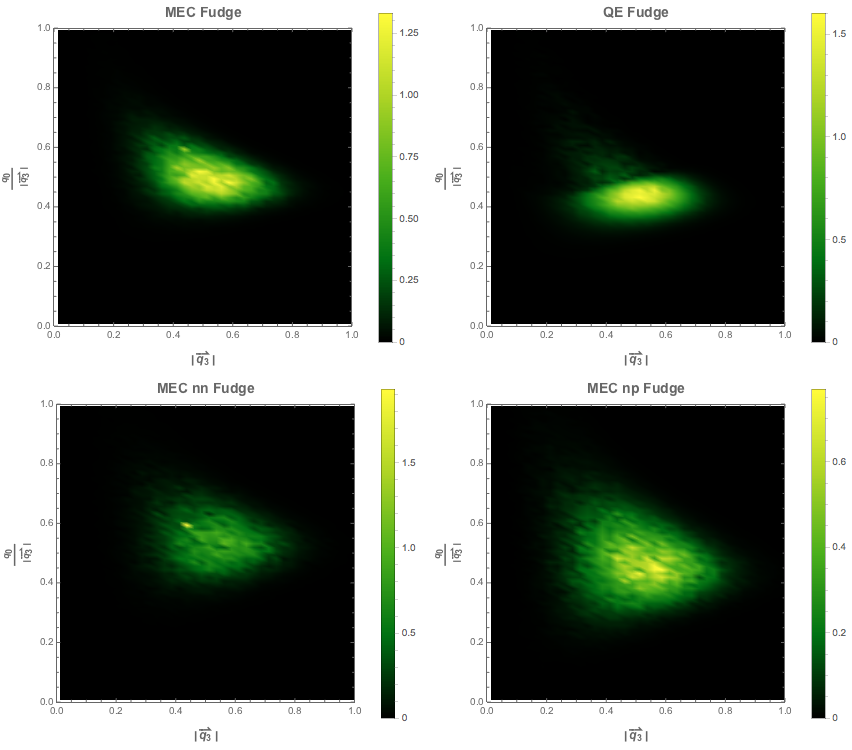
\includegraphics[width=\textwidth]{graphics/Fudges.png}
%\end{dunefigure}

%\begin{dunefigure}[Added differential $d^2\sigma/dq_0dq_3$ crosssections for $\anu$s averaged over the MINERvA flux]{fig:mnvTunesNubar}
%{The added differential $d^2\sigma/dq_0dq_3$ cross sections averaged over the MINERvA flux for antineutrinos in units of $10^{-38}/cm^2/GeV^2$ for the default \minerva tune and the three systematic variations.  Each is in good agreement with the \minerva "low recoil" data in \minerva's antineutrino~\cite{Gran:2018fxa} beam. \todo{Fix titles/label/update MnvTunes plots 2/2}}
%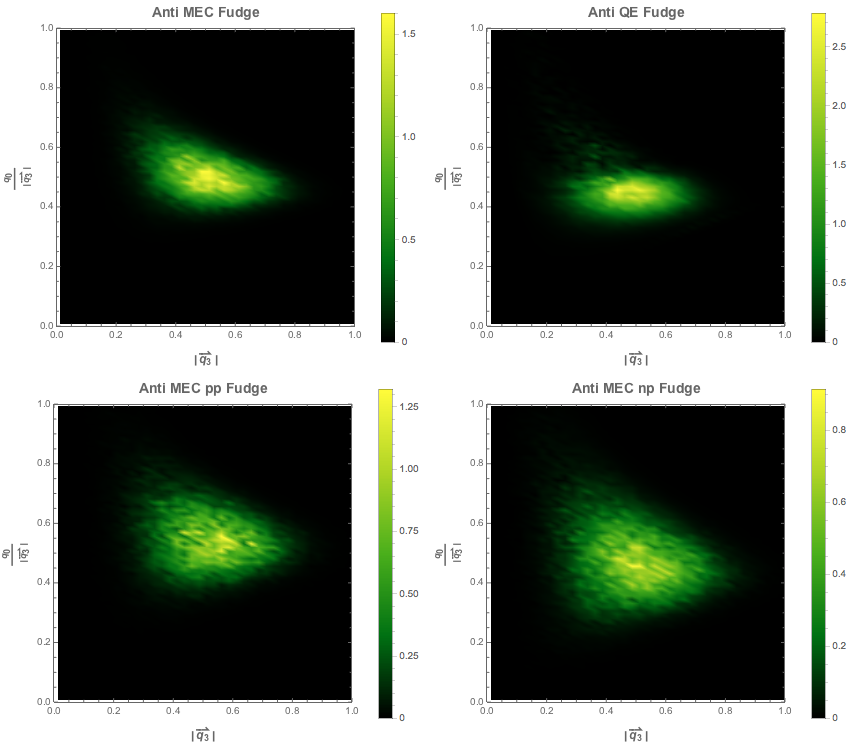
\includegraphics[width=\textwidth]{graphics/antiFudges.png}
%\end{dunefigure}

The rates for $1p1h$ and $2p2h$ processes could be different on argon and carbon targets.  There is little neutrino scattering data to inform this, but there are measurements of short-ranged correlated pairs from electron scattering on different nuclei~\cite{Colle:2015ena}.  These measurements directly constrain $2p2h$ from short range correlations, although the link to dynamical sources like meson exchange current processes (MEC) is less direct. Interpolation of that data in $A$ (Nucleon number) suggests that scaling from carbon relative to the naive $\propto A$ prediction for $2p2h$ processes would give an additional factor of $1.33\pm 0.13$ for $np$ pairs, and $0.9\pm 0.4$ for $pp$ pairs.
\dword{genie}'s prediction for the ratio of $2p2h$ cross-sections in $\text{Ar}^{40}/\text{C}^{12}$ for neutrinos varies slowly with neutrino energy in the DUNE energy range: from $3.76$ at $1$~GeV to $3.64$ at $5$~GeV. The ratio for antineutrino cross sections is consistent with $3.20$ at all DUNE energies. Since the ratio of $A$ for $\text{Ar}^{40}/\text{C}^{12}$ is $3.33$, this is consistent with the ranges suggested above by the measured $pp$ and $np$ pair scaling.  A dedicated study by the SuSA group using their own theoretical model for the relevant MEC process also concludes that the transverse nuclear response (which drives the $\nu-A$ MEC cross section) ratio between $\text{Ca}^{40}$ (the isoscalar nucleus with the same $A$ as $\text{Ar}^{40}$) and $\text{C}^{12}$ is $3.72$ \cite{Amaro:2017eah}. We conclude that we should vary \dword{genie}'s Valencia model based prediction, including the \minerva tune, for $2p2h$ by $\sim 20\%$ to be consistent with the correlated pair scaling values above. This is done independently for neutrino and antineutrino scattering.

The \minerva tune may be $E_\nu$ dependent. \minerva separated its data into an $E_\nu<6$~GeV and an $E_\nu>$6~GeV piece, and sees no dependence with a precision of better than $10\%$~\cite{Rodrigues:2015hik}.  The mean energy of the $E_\nu<6$~GeV piece is roughly $\left< E_\nu\right>\approx 3$~GeV.  In general, an exclusive cross-section will have an energy dependence $\propto \frac{A}{E_\nu^2}+\frac{B}{E_\nu}+C$~\cite{llewelyn-smith}; therefore, unknown energy dependence may be parametrized by an {\em ad hoc} factor of the form $1/\left(1+ \frac{A^{'}}{E_\nu^2 }+\frac{B^{'}}{E_\nu}\right)$.  The \minerva constraints suggest $A^{'}<0.9$~GeV$^2$ and $B^{'}<0.3$~GeV.  The variations for neutrinos and antineutrinos could be different since this is an effective modification. Ideally this energy dependent factor would only affect the \minerva tune, but practically, becasue of analysis framework limitations already discussed, this is not possible. As a result, this energy dependent factor is applied to all true $2p2h$ events.

\subsubsection{Single pion production uncertainties}
\dword{genie} uses the Rein-Sehgal model for pion production. Tunes to $D_2$ data have been performed, both by the \dword{genie} collaboration itself and in subsequent re-evaluations~\cite{Rodrigues:2016xjj}; we use the latter tune as our base model. For simplicity of implementation, the `v2.8.2 (no norm.)' results are used here. Ideally the `v2.8.2 (RES)' would have been used, but the practical effect of this choice on the quoted sensitivities is expected to be small.

\minerva single pion production data~\cite{Altinok:2017xua,McGivern:2016bwh,Eberly:2014mra} indicates disagreement at low $Q^2$ which may correspond to an incomplete nuclear model for single pion production in the generators. A similar effect was observed at MINOS\cite{minos_pi_q2} and \nova implements a similar correction in analyses~\cite{nova_2018}.
A fit to \minerva data~\cite{StowellThesis} measured a suppression parameterized by
\begin{align}
R(Q^2<x_3) & = \frac{R_{2} (Q^2-x_1)(Q^2-x_3)}{(x_2-x_1)(x_2-x_3)} \notag\\
             & + \frac{(Q^2-x_1)(Q^2-x_2)}{(x_3-x_1)(x_3-x_2)}  \\
W(Q^{2}) &= 1-(1-R_{1})(1-R(Q^{2}))^{2}
\end{align}
where $R_{1}$ defines the magnitude of the correction function at the intercept, $x_{1}=0.0$. $x_{2}$ is chosen to be $Q^2=0.35\text{ GeV}^2$ so that $R_{2}$ describes the curvature at the centre point of the correction. The fit found $R_1\approx0.3$ and $R_2\approx0.6$. The correction is applied to events with a resonance decay inside the nucleus giving rise to a pion, based on \dword{genie} event information.

An improved Rein-Seghal-like resonance model has recently been developed~\cite{minoo} which includes a non-resonant background in both $I=\frac{1}{2}$ and $I=\frac{3}{2}$ channels and interference between resonant-resonant and resonant-non-resonant states. %Additionally, it uses the full resonance continuum to calculate the pion-nucleon ejection kinematics, which the Rein-Sehgal model only uses $\Delta(1232)$ for.
It also improves on the Rein-Sehgal model in describing the outgoing pion and nucleon kinematics using all its resonances.
%The anti-neutrino cross-section is between 200-400\% larger than for the Rein-Sehgal model, in contention with data from MINERvA\cite{McGivern:2016bwh}.
%Implementation: Template weighting in $(W, Q^2, E_\nu)$ or $(q_0, q_3, E_\nu)$. Uncertainty: Excursion set to cover difference between the MK model and current Rein-Sehgal model.
A template weighting in $(W, Q^2, E_\nu)$ is implemented to cover the differences between the two models as a systematic uncertainty. The weighting also suppresses \dword{genie} 'non-resonant pion production' events (deep inelastic scattering events with $W<1.7\text{ GeV}$) as the new model already includes the non-resonant contribution coherently. At the time of writing, problems in the anti-neutrino prediction of this model had been recently found, and an updated implementation was not available, as a result the weighting is only applied to true muon-neutrino charged-current resonant pion production interactions.

Coherent inelastic pion production measurements on carbon are in reasonable agreement with the \dword{genie} implementation of the Berger-Sehgal model~\cite{Mislivec:2017qfz}.  The process has not been measured at high statistics in argon. While coherent interactions provide a very interesting sample for oscillation analyses, they are a very small component of the event rate and selections will depend on the near detector configuration. Therefore we do not provide any evaluation of a systematic uncertainty for this extrapolation or any disagreements between the Berger-Sehgal model and carbon data.

\subsubsection{Other hard scattering uncertainties}
\nova oscillation analyses~\cite{nova_2018} have found the need for excursions beyond the default \dword{genie} uncertainties to describe their single pion to deep inelastic scattering (DIS) transition region data.  Following suit, we drop \dword{genie}'s default ``Rv[n,p][1,2]pi'' knobs and instead implement separate, uncorrelated uncertainties for all perturbations of 1, 2, and $\geq 3$ pion final states, CC/NC, neutrinos/anti-neutrinos, and interactions on protons/neutrons, with the exception of CC neutrino 1-pion production, where interactions on protons and neutrons are merged, following \cite{Rodrigues:2016xjj}. This leads to 23 distinct uncertainty channels ([3 pion states] x [n,p] x [nu/anti-nu] x [CC/NC] - 1), all with a value of 50\% for $W \leq 3$ GeV.  For each channel, the uncertainty drops linearly above $W = 3$ GeV until it reaches a flat value of 5\% at $W = 5$ GeV, where external measurements better constrain this process.

\subsubsection{Final state interaction uncertainties}\label{sec:fsi}
\dword{genie} includes a large number of final state uncertainties to its $hA$ final state cascade model which are summarized in Table~\ref{table:HadTranspKnobs}.  These uncertainties have been validated in neutrino interactions primarily on light targets such as carbon, but there is very little data available on argon targets.
The lack of tests against argon targets is difficult to address directly because there are many possible \dword{fsi} processes that could be varied, but it would nevertheless be a mistake not to put some degree of freedom in the model to address this.

The \dword{fsi} uncertainties are parameterized in terms of a effect on the primary experimental observable. The DUNE detectors seek to keep all observed final states as signal samples, so it is natural to consider the effect of a variation on the reconstructed energy.  The DUNE detector will measure a recoil quantity which will need to be mapped to the true energy loss from the leptonic system, or $q_0$.  In the absence of sophisticated particle flow calorimetry\footnote{Such a sophisticated particle flow reconstruction will eventually follow but is not yet available at this stage of the experimental development} a good approximation to the measured recoil energy is the $E_\text{avail}$---the recoil energy less the rest mass of charged pions and the kinetic energy of any produced neutrons. \dword{fsi} will alter the calorimetric factor ($\mathcal{C}_\textsc{f} = E_{avail}/q_0$) by changing the fraction of recoil energy in neutrons and charged pions while preserving the total cross section.
The uncertainty parameterization developed here looks at how \dword{fsi} alters $E_{avail}/q_0$ in carbon, and applies an arbitrary 30\% fraction of this shift to the default prediction on argon.  Event weights as a function of $(q_3,q_0,\mathcal{C}_\textsc{f})$ are calculated such that the total cross section in each $(q_3,q_0)$ bin is conserved, while the first and second moments of the $\mathcal{C}_\textsc{f}$ distribution are modified. The shifts are calculated for charged-current events and are split into neutrino/anti-neutrino and further by interaction mode into $1p1h$, $2p2h$, resonant and DIS interactions. In this analysis effect of this parameter is fully correlated between neutrino and anti-neutrino interactions.

\subsubsection{Missing visible energy mock data study}
\label{sec:nu_osc__nuint__MissingEnergyMDS}
%\fixme{This needs an introduction}
The mock data set considered here is generated by scaling down the energy deposits due to protons by 20\%, under the assumption that this missing energy is instead carried by some other, unobserved particles, such as neutrons:
\begin{equation}
E_{\rm proton}^{dep} \rightarrow E_{\rm proton}^{\prime dep} = 0.8 \times E_{\rm proton}^{dep} \, .
\end{equation}
%\todo{It should probably be noted here that we need to use different FarDet recon to do this because no one knows how the CVN assigns energy and we didn't have resources to run a parallel production.}
This propagates to the reconstructed neutrino energy as:
\begin{equation}
E_{\rm rec} \rightarrow E_{\rm rec}^{\prime} = E_{\rm rec} - 0.2 \times E_{\rm proton}^{dep} \, .
\label{eqn:nu_osc__nuint__MissingEnergyMDS__ERec}
\end{equation}

%\todo{Introduce the event weighting procedure here: A weighting function is applied to recover agreement with the nominal on-axis sample detector observables.}

The modified proton energy systematic uncertainty is treated as a discrete alternate model, to test the entire chain of oscillation analysis robustness to an alternate assumption on the true--observed energy relationship in the interaction model. The mock data is prepared by varying the reconstructed energy of each selected event according to \eqref{eqn:nu_osc__nuint__MissingEnergyMDS__ERec} and a cross section modification is applied as an event weight.


\subsubsection{Neutrino flavor dependent uncertainties}
The cross sections include terms proportional to lepton mass, which are significant contributors at low energies where quasielastic processes dominate.  Some of the form factors in these terms have significant uncertainties in the nuclear environment.  Ref.~\cite{Day-McFarland:2012} ascribes the largest possible effect to the presence of poorly constrained second-class current vector form factors in the nuclear environment, and proposes a variation in the cross section ratio of $\sigma_\mu/\sigma_e$ of $\pm 0.01/{\rm\textstyle Max}(0.2~{\rm\textstyle GeV},E_\nu)$ for neutrinos and $\mp 0.018/{\rm\textstyle Max}(0.2~ {\rm\textstyle GeV},E_\nu)$ for anti-neutrinos.  Note the anticorrelation of the effect in neutrinos and antineutrinos.

In addition, radiative Coulomb effects may also contribute, which for T2K is of order $\pm5$ MeV shifts in reconstructed lepton momentum.  Like the second class current effect in the cross section, it flips sign between neutrinos and antineutrinos and is significant only at low energies.  This effect is not implemented herein.

Finally, some electron neutrino interactions occur at four momentum transfers where a corresponding muon neutrino interaction is kinematically forbidden, therefore the nuclear response has not been constrained by muon neutrino cross section measurements.  This region at lower neutrino energies has a significant overlap with the Bodek-Ritchie tail of the Fermi gas model. There are significant uncertainties in this region, both from the form of the tail itself, and from the lack of knowledge about the effect of RPA and $2p2h$ in this region. The allowed phase space in the presence of non-zero lepton mass is $E_\nu-\sqrt{\left( E_\nu-q_0\right) ^2-m_l^2}\leq q_3\leq E_\nu+\sqrt{\left( E_\nu-q_0\right) ^2-m_l^2}$. Here, a 100\% variation is allowed in the phase space present for $\nu_e$ but absent for $\nu_\mu$.

A similar prescription cannot applied for differences between interactions of $\nu_\mu$ and $\nu_\tau$ because the $\tau$ mass scale is of the same order of magnitude as the neutrino energies, and is thus a leading effect. No specific uncertainties were developed for $\nu_\tau$ interactions as there is little theoretical guidance, but it should be noted that this constitutes an underestimation of the errors for analyses including selected $\nu_\tau$ events.

\subsubsection{Summary of interaction model uncertainties}

The complete set of interaction model uncertainties includes most of the suggested \dword{genie} default uncertainties (Tables~\ref{table:NuXSecKnobs}, %\ref{table:HadronzKnobs},
\ref{table:HadTranspKnobs}),  modified uncertainties (Table~\ref{}), or new uncertainties developed for this effort (Table~\ref{tab:nuintsystlist}).

\begin{table}[htb]
\center
\global\long\def\arraystretch{1.75}
\scalebox{0.9}{
\begin{tabular}{llr|l}
\hline
$x_{P}$  & Description of $P$  & $P_\textsc{cv}$ & $\delta{P}/{P}$  \tabularnewline
\hline
&\textbf{Quasielastic}&&\tabularnewline
$x_{M_{A}}^{CCQE}$ & Axial mass for CCQE & & ${}^{+0.25}_{-0.15}$~GeV \tabularnewline
$x_{VecFF}^{CCQE}$  & Choice of CCQE vector form factors (BBA05 $\leftrightarrow$ Dipole)  &  & N/A \tabularnewline
$x_{kF}^{CCQE}$  & Fermi surface momentum for Pauli blocking &   & $\pm$30\% \tabularnewline
&\textbf{Low $\mathbf{W}$}&&\tabularnewline
$x_{M_{A}}^{CCRES}$ & Axial mass for CC resonance & 0.94 & $\pm$0.05~GeV \tabularnewline
$x_{M_{V}}^{CCRES}$  & Vector mass for CC resonance &  & $\pm$10\% \tabularnewline
$x_{\eta\ BR}^{\Delta Decay}$  & Branching ratio for $\Delta\rightarrow\eta$ decay &   & $\pm$50\% \tabularnewline
$x_{\gamma\ BR}^{\Delta Decay}$  & Branching ratio for $\Delta\rightarrow\gamma$ decay &   & $\pm$50\% \tabularnewline
$x_{\theta_{\pi}^{\Delta Decay}}$  & $\theta_{\pi}$ distribution in decaying $\Delta$ rest frame (isotropic $\rightarrow$ RS) &   & N/A \tabularnewline
&\textbf{High $\mathbf{W}$}&\tabularnewline
$x_{A_{HT}^{BY}}^{DIS}$  & $A_{HT}$ higher-twist param in BY model scaling variable $\xi_{w}$  &   & $\pm$25\% \tabularnewline
$x_{B_{HT}^{BY}}^{DIS}$  & $B_{HT}$ higher-twist param in BY model scaling variable $\xi_{w}$  &  & $\pm$25\% \tabularnewline
$x_{C_{V1u}^{BY}}^{DIS}$  & $C_{V1u}$ valence GRV98 PDF correction param in BY model  &  & $\pm$30\% \tabularnewline
$x_{C_{V2u}^{BY}}^{DIS}$  & $C_{V2u}$ valence GRV98 PDF correction param in BY model  &  & $\pm$40\% \tabularnewline
% Excluded as they are too slow, extra Npi dials give significant normalization freedom to DIS pion production
% $x_{x_{F}^{AGKY1\pi}}^{DIS}$  & Vary the $x_{F}$ distribution for 1$\pi$ DIS produced by AGKY &  & $\pm$20\% \tabularnewline
% $x_{p_{T}^{AGKY1\pi}}^{DIS}$  & Vary the $p_{T}$ distribution for 1$\pi$ DIS produced by AGKY &  & $\pm$3\% \tabularnewline
&\textbf{Other neutral current}&&\tabularnewline
$x_{M_{A}}^{NCEL}$  & Axial mass for NC elastic  &  & $\pm$25\% \tabularnewline
$x_{\eta}^{NCEL}$  & Strange axial form factor $\eta$ for NC elastic  &  & $\pm$30\%  \tabularnewline
$x_{M_{A}}^{NCRES}$  & Axial mass for NC resonance & &$\pm$10\% \tabularnewline
$x_{M_{V}}^{NCRES}$  & Vector mass for NC resonance & &$\pm$5\% \tabularnewline
&\textbf{Misc.}&&\tabularnewline
$x_{FZ}$  & Vary effective formation zone length &  & $\pm$50\% \tabularnewline
\hline
\end{tabular}
}% scalebox
\\[2pt]
\caption{Neutrino interaction cross-section systematic parameters considered
in \dword{genie}. \dword{genie} default central values and uncertainties are used for all parameters except $x_{M_{A}}^{CCRES}$. Missing \dword{genie} parameters were omitted where uncertainties developed for this analysis significantly overlap with the supplied \dword{genie} freedom, the response calculation was too slow, or the variations were deemed unphysical.
}
\label{table:NuXSecKnobs}
\end{table}

% Central values tunes
% BeRPA, MACCRES, Nonresonant background 1pi, MINERvA 2p2h tune
\begin{table}[htb]
\center
\global\long\def\arraystretch{1.75}
\scalebox{0.9}{
\begin{tabular}{ll|l}
\hline
$x_{P}$  & Description of $P$ & $P_{CV}$  \tabularnewline
\hline
&\textbf{Quasielastic} & \tabularnewline
BeRPA & Random Phase Approximation tune & $A: 0.59$ \tabularnewline
& $A$ controls low $Q^2$, $B$ controls low-mid $Q^2$ & $B: 1.05$ \tabularnewline
& $D$ controls mid $Q^2$, $E$ controls high $Q^2$ fall-off & $D: 1.13$ \tabularnewline
& $U$ controls transition from polynomial to exponential & $E: 0.88$ \tabularnewline
& & $U: 1.20$ \tabularnewline
&\textbf{2p2h}&\tabularnewline
MINERvA 2p2h tune & $q0,q3$ dependent correction to 2p2h events&\\
&\textbf{Low $\mathbf{W}$ single pion production} & \tabularnewline
$x_{M_{A}}^{CCRES}$ & Axial mass for CC resonance in \dword{genie}& $0.94$ \tabularnewline
Non-res CC1$\pi$ norm. & Normalisation of CC1$\pi$ non-resonant interaction & $0.43$  \tabularnewline
\hline
\end{tabular}
}% scalebox
\\[2pt]
\caption{Neutrino interaction cross-section systematic parameters which receive a central-value tune}
\label{table:NuXSecKnobs_Central}
\end{table}


\begin{table}[htb]
\center

\global\long\def\arraystretch{1.75}
% enlarge line spacing
\begin{tabular}{llll}
\hline
$x_{P}$  & Description of $P$  & $\delta{P}/{P}$  & \tabularnewline
\hline
% $x_{mfp}^{N}$  & Nucleon mean free path (total rescattering probability)  & $\pm$20\%  & \tabularnewline
$x_{cex}^{N}$  & Nucleon charge exchange probability  & $\pm$50\%  & \tabularnewline
$x_{el}^{N}$  & Nucleon elastic reaction probability  & $\pm$30\%  & \tabularnewline
$x_{inel}^{N}$  & Nucleon inelastic reaction probability  & $\pm$40\%  & \tabularnewline
$x_{abs}^{N}$  & Nucleon absorption probability  & $\pm$20\%  & \tabularnewline
$x_{\pi}^{N}$  & Nucleon $\pi$-production probability  & $\pm$20\%  & \tabularnewline
% $x_{mfp}^{\pi}$  & $\pi$ mean free path (total rescattering probability)  & $\pm$20\%  & \tabularnewline
$x_{cex}^{\pi}$  & $\pi$ charge exchange probability  & $\pm$50\%  & \tabularnewline
$x_{el}^{\pi}$  & $\pi$ elastic reaction probability  & $\pm$10\%  & \tabularnewline
$x_{inel}^{\pi}$  & $\pi$ inelastic reaction probability  & $\pm$40\%  & \tabularnewline
$x_{abs}^{\pi}$  & $\pi$ absorption probability  & $\pm$20\%  & \tabularnewline
$x_{\pi}^{\pi}$  & $\pi$ $\pi$-production probability  & $\pm$20\%  & \tabularnewline
\hline
\end{tabular}\\[2pt] \caption{The intra-nuclear hadron transport systematic parameters implemented in \dword{genie} with associated uncertainties considered in
this work. Note that the 'mean free path' parameters are omitted for both N-N and $pi$-N interactions as they produced unphysical variations in observable analysis variables. Table adapted from Ref~\cite{}% https://arxiv.org/pdf/1510.05494.pdf
}


\label{table:HadTranspKnobs}
\end{table}

Table~\ref{tab:nuintsystlist} separates the interaction model parameters into three categories based on their treatment in the analysis:
\begin{itemize}
\item Category 1:  On-axis near detector data is expected to constrain these parameters; the uncertainty is implemented in the same way in near and far detectors.
\item Category 2: These uncertainties are implemented in the same way in near and far detectors, but on-axis data alone is not sufficient to constrain these parameters. We use two sub-categories. The first category (2A) corresponds to interaction effects which may be difficult to disentangle from detector effects. The best example of this is the $E_b$ parameter, which may be degenerate with the energy scale of the near detector; this may be constrained with electron scattering and/or thoughtful alternate projections of near detector data (Section~\ref{sec:nu-osc-06}). The second category (2B) corresponds to parameters where off-axis samples, described in Section~\ref{sec:nu-osc-06}, will likely constrain these effects significantly.
%An observed constraint from the near detector on-axis position alone should be viewed with suspicion and be scrutinized for why it provides constraint. Previous studies of conventional near detectors indicate that constraint of (true energy) systematic uncertainties is difficult or artificial.
%It is expected additional developments in the ND group (e.g. DUNE PRISM~\cite{docdbDUNEPRISM}\fixme{Need to define off-axis angles here/make more general as term not introduced yet.}, scintillator detector neutron information) may provide a reasonable mechanism to constrain these parameters. If we find no reasonable mechanism or artificial constraint, we would iterate with ND groups to adjust the treatment. As an example, a workaround would be to force these parameters to be uncorrelated between near and far detector.
\item Category 3: Uncertainty should be implemented only in the far detector (e.g. as $\nu_e$ and $\overline{\nu}_e$ rates are  small at the near detector).  Near detector data is not expected to constrain such parameters.
\end{itemize}
All \dword{genie} uncertainties (original or modified) are all treated as Category 1.

%\afterpage{
%\begin{landscape}
%\mbox{}\vfill
\begin{table}[ptb]
\scalebox{0.9}{
\begin{tabular}{lccc}\hline
Uncertainty & Mode & Description & Category  \\  \hline \hline
BeRPA & 1p1h/QE & RPA/nuclear model suppression &  1  \\  \hline
% $E_b$ & 1p1h/QE & Shift in nuclear model removal energy  &  2A   \\  \hline %2
MnvTune1 & 2p2h & Strength into (nn)pp only &  1 \\  \hline
% MnvaTune2 & 2p2h  & Strength into np pairs only &  1 \\  \hline
MnvTuneCV & 2p2h & Strength into 2p2h  &  1 \\  \hline
MnvTune2 & 1p1h/QE & Strength into 1p1h  &  1 \\  \hline
ArC2p2h & 2p2h Ar/C scaling & Electron scattering SRC pairs & 1 \\ \hline
$E_{2p2h}$ & 2p2h & 2p2h Energy dependence  &  2B \\  \hline
Low $Q^2$ $1\pi$ & RES & Low $Q^2$ (empirical) suppression &   1 \\  \hline
MK model & $\nu_\mu$ CC-RES & Alternate strength in W &   1 \\  \hline
CC Non-resonant $\nu\rightarrow\ell+1\pi$ & $\nu$ DIS & Norm. for $\nu+n/p\rightarrow\ell+1\pi$ (\it{c.f.}\ref{Rodrigues:2016xjj}) & 1 \\ \hline
Other Non-resonant $\pi$ & $N\pi$ DIS & Per-topology norm. for $1<W<5$ GeV. & 1 \\ \hline
$E_{avail}/q_0$ & all & Extreme \dword{fsi}-like variations  &  2B \\
\hline
Modified proton energy & all & 20\% change to proton E &  2B \\
\hline
$\nu_\mu\to\nu_e$ & $\nu_e$/$\overline{\nu}_e$ & 100\% uncertainty in $\nu_e$ unique phase space &  3 \\ \hline
$\nu_e$/$\overline{\nu}_e$ norm & $\nu_e$,$\overline{\nu}_e$ & Ref.~\cite{Day-McFarland:2012}  &  3 \\
\hline
\hline
\end{tabular}
} % scalebox
\caption{List of extra interaction model uncertainties in addition to those provided by \dword{genie}.}
\label{tab:nuintsystlist}
\end{table}
%\vfill
%\end{landscape}
%}

%\subsubsection{Uncertainties not accounted for in this framework}
%% KM - Merged with introduction which seems natural to raise caveats. Other cases here are described well in the text.

%As previously noted, there are cross section variations which are not easily accounted for in the framework that has been developed for the DUNE TDR.  Alternate initial state models are extremely difficult to study, and in many cases not implemented within the GENIE framework.  Alternate final state interaction models do exist within GENIE, but one can not reweight between final state interaction models.

%Another category of systematic uncertainty not considered are ones that are, in principle, easily handled within this framework, but are not ready for the TDR.  Those include studies of Coulomb corrections, particularly as they relate to flavor dependent uncertainties, use of the $z$-expansion to describe weak form factors of nucleons, and uncertainties on coherent inelastic pion production which is a subleading process.

%Table~\ref{tab:mds} lists a set of possible mock data studies which would address some of these missing systematic uncretainties. Ideally, the suite of uncertainties provided in the proposed model should appropriately cover these scenarios. However, if bias or decreased coverage of oscillation parameters is observed outside of the coverage of the reweightable systematics, then the final contours should be appropriately adjusted.

%\begin{table}
%\begin{tabular}{lcc}\hline
%\hline
%NEUT SF & QE+FSI & SF with different FSI, no 2p2h  \\  \hline
%NuWro & all+FSI &  Similar underlying model with different FSI  \\  \hline
%%GENIE & G18\_10a &  Alternate GENIE models \\ \hline
%GENIE hN2015 & all & Same base model as production with alternate FSI model \\ \hline
%z-expansion & QE & Alternate non-dipole form factors   \\  \hline
%DUNE PRISM & all & Probes $E_{rec}$-$E_{true}$ response function.   \\
%\end{tabular}
%\caption{List of alternate models to be tested in the analysis (``mock data studies'')}
%\label{tab:mds}
%\end{table}
